\section{\deltaray Corrections}
\label{sec:corr}
\subsection{Backgrounds}
	Gamma conversion to electron positron pairs can produce electrons within the energy window. This is an irreducible background to our measurement. The energy spectrum for produced electrons and positrons should be symmetric. Identifying positrons created in the beam pipe region and subtracting them from the electron spectrum allows us to statistically subtract the effects of gamma conversion from our measurement. The Monte Carlo simulated positron distribution agrees with the 7\% data sample shown in figure 
	\ref{fig:posdist}.
	\begin{figure}[htb]
		\centering
		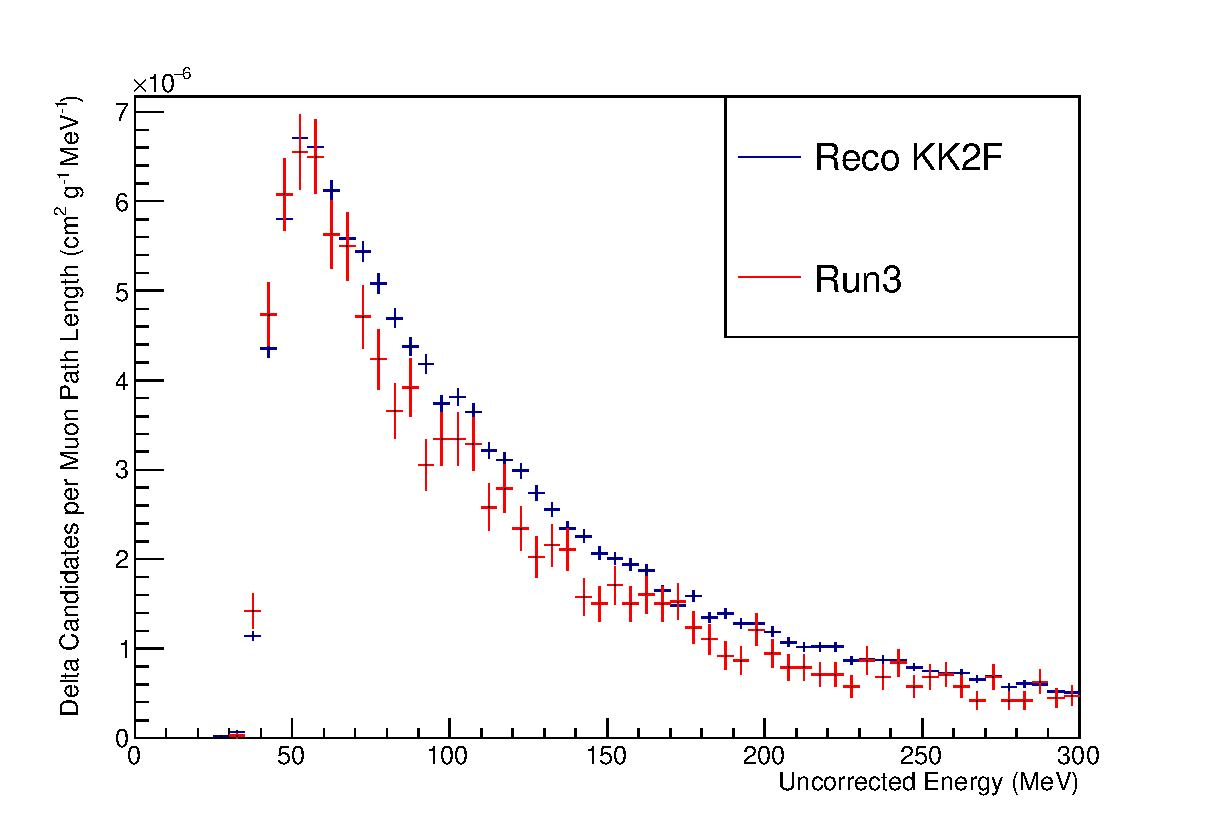
\includegraphics[scale=0.5]{figures/posdist.eps}
		\caption{Positron distribution after applying delta ray cuts for both Monte Carlo and Run 3 data. Shown uncertainties are purely statistical.}
		\label{fig:posdist}
	\end{figure}	
	
	Other backgrounds to the measurement are much smaller and are largely removed by data cuts. These will be further removed by statistically subtracting the expected amounts from Monte Carlo simulations.

\subsection{Acceptance and Efficiency}
	\babar geometric acceptance is taken into account by the selections on the muons. All muons are selected to have 4 SVT hits and 12 Drift Chamber Hits. This requires that the \deltarays are occurring in the central region of the detector. The geometric selection cuts are performed using local reconstructed variables for the muon track.
	
	The \babar detector has a varying efficiency which changes with energy. The efficiency probability is calculated for each energy bin using the Monte Carlo truth. The number of true detected \deltarays at each energy is divided by the total number of true \deltarays at that energy. The efficiency for the beam pipe is shown in figure 
	\ref{fig:BPeff}. This is then used to correct the measured distribution by dividing the energy corrected \deltaray distribution by the detector efficiency bin by bin.
	\begin{figure}[htb]
		\centering
		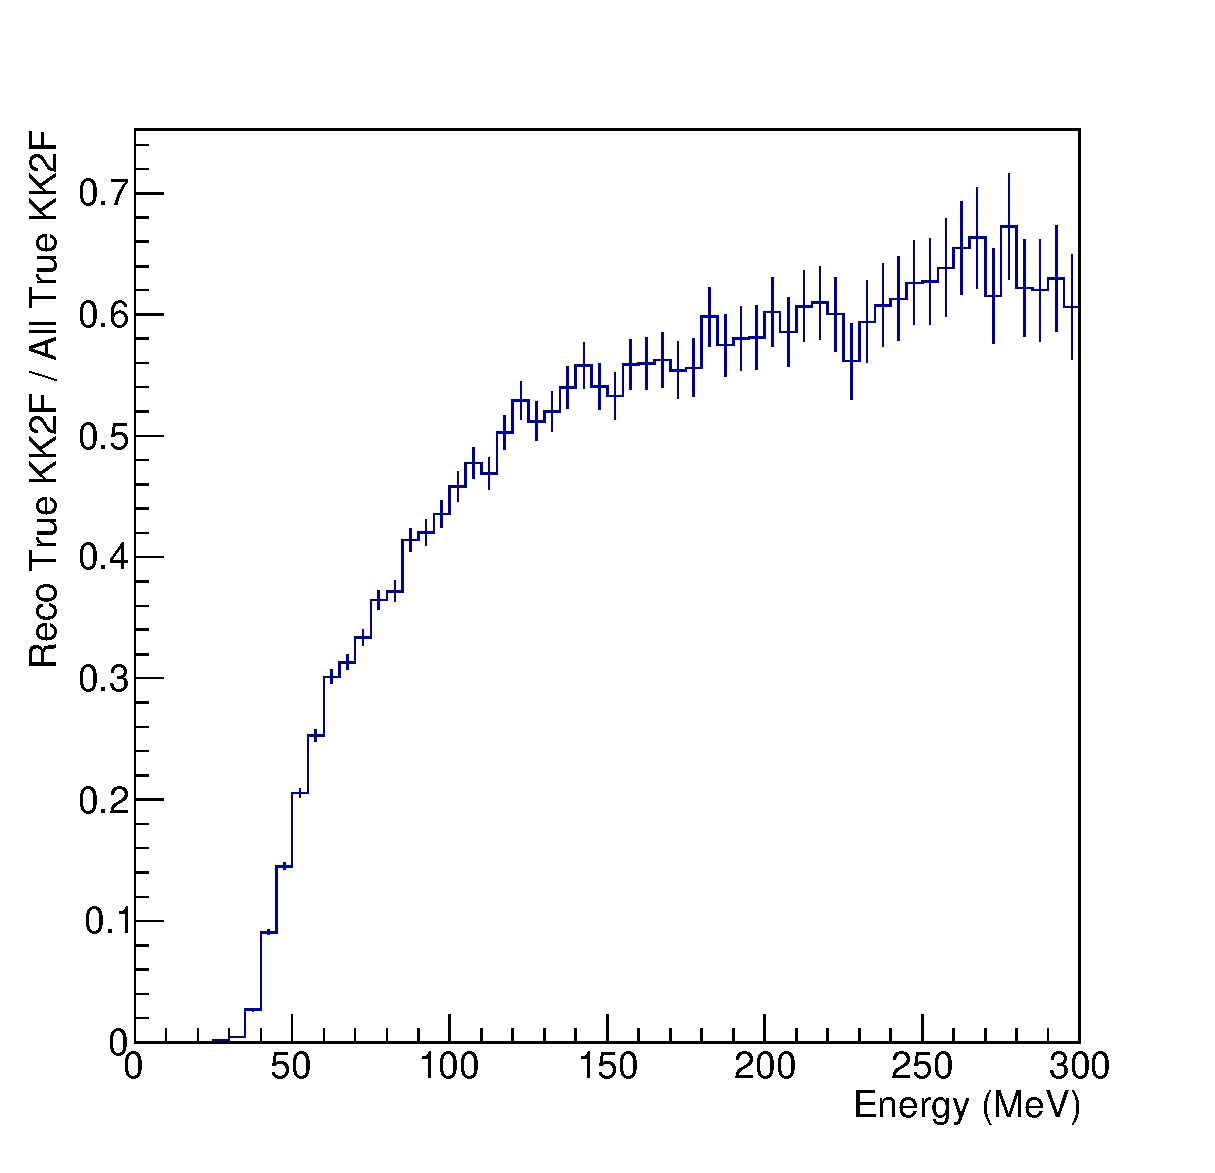
\includegraphics[scale=0.5]{figures/Efficiency.eps}
		\caption{Reconstruction efficiency for true delta rays created in beam pipe.}
		\label{fig:BPeff}
	\end{figure}

\subsection{Energy Correction}
	There is a small effect of energy smearing from the detector on the selected \deltarays. This is partially due to smearing effects, and to bremsstrahlung \ref{fig:BPsmear}. This effect can be correcting using an unfolding  process. This is performed using the ROOT class TSVDUnfold (**include reference), which uses the Monte Carlo simulation of the true distribution and detected distribution. The energy smearing matrix is inverted with a regularization factor for the Singular Value Decomposition. 
	\begin{figure}[htp]
		\centering
		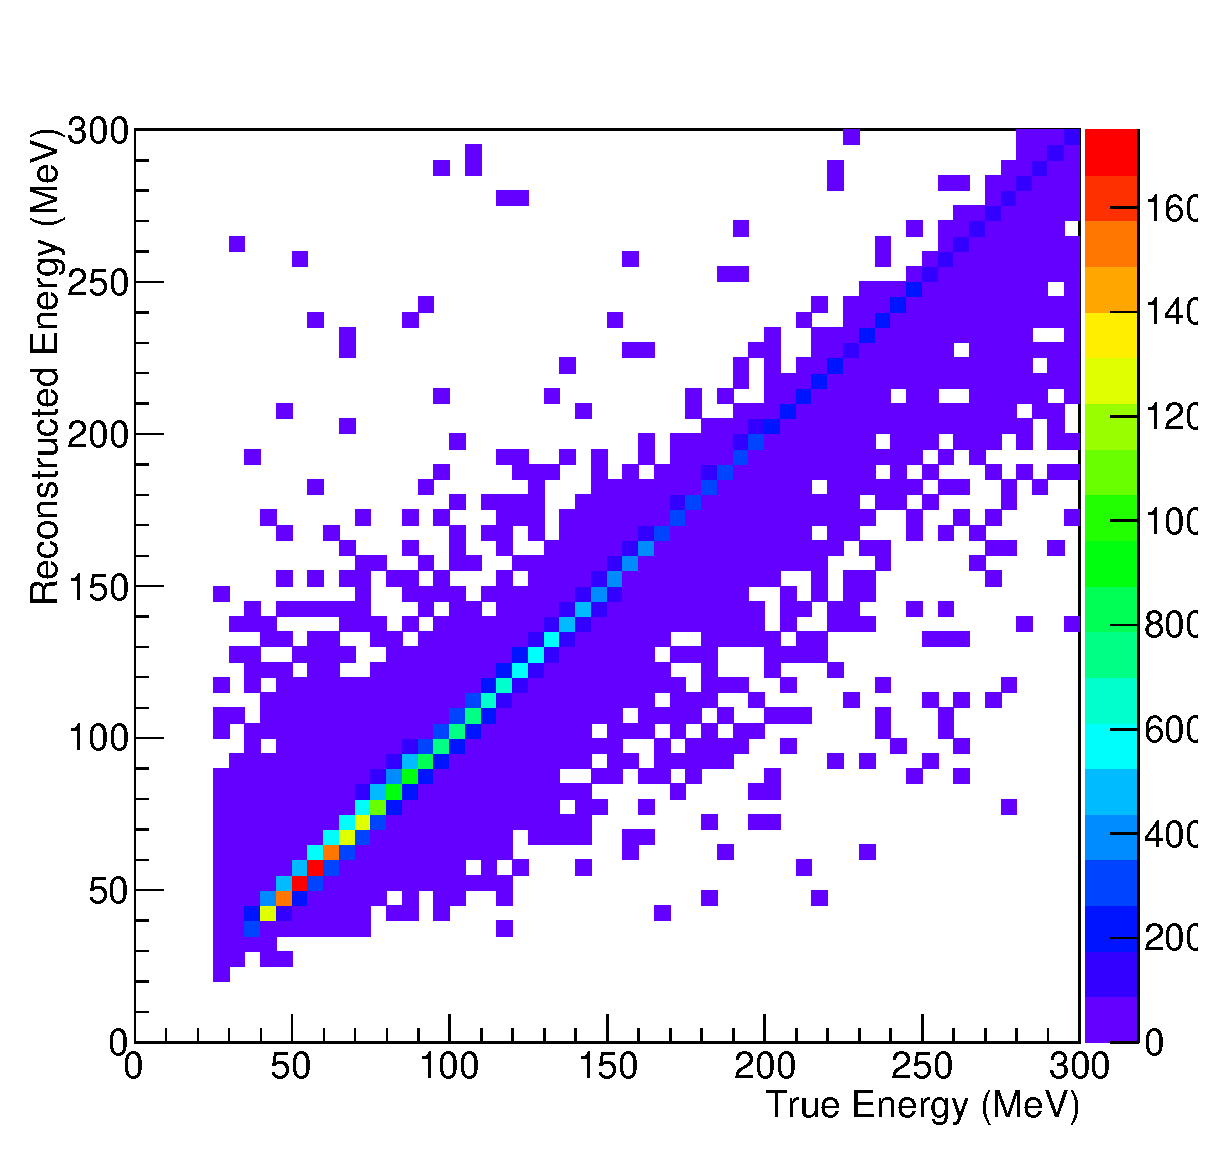
\includegraphics[scale=0.5]{figures/Energy_Smearing.eps}
		\caption{Reconstructed energy of true delta rays versus the true energy of the delta rays. This smearing effect can be corrected using a matrix inversion method.}
		\label{fig:BPsmear}
	\end{figure}

	This process was tested on the Monte Carlo data. First we separated every other event into a training sample and a test sample. Then we treated the training sample as the Monte Carlo truth and used it to perform the correction on the test sample’s detected distribution. This Provided a distribution of corrected \deltarays that agreed with the Monte Carlo truth for the test sample.

\subsection{Material Transit}
	To turn the \deltaray distribution into a physical cross section we need to scale it to get physical units. The scaling factor is the density of the beam pipe multiplied by the sum of the path lengths for all selected muons that pass through the beam pipe. This is calculated from the prescaled sample where selections are placed on the \deltarays, only requirement is two muon tracks. Dividing the thickness of the beam pipe by the dot product of the muon track with the normal vector of the beam pipe provides the path length through the material.
\subsection{Material Misidentification}
	The material of \deltaray production is identified using the POCA position of the \deltaray track. This value is calculated using the reconstructed track data and can lead to mislabeling. The values shown in table \ref{tab:Xfeed} show this is a small effect for most regions of the detector. This becomes important in calculating the cross section for the CST and DCH regions of the detector as there is about 20\% crossfeed. All other detector regions have crossfeed values at about 1\%.
	\begin{table}[htb]
		\begin{center}
			\caption{Material Misidentification Matrix}
			\label{tab:Xfeed}
			\begin{tabular}{||c|c|c|c|c|c|c||}
				\hline
				\hline
				& BP & SVT1 & SVT2-5 & ST & Dch & other\\
				\hline
				BP & 0.99394 & 0.00071 & 0.00404 & 0 & 0 & 0.00129\\
				\hline
				SVT1 & 0.05299 & 0.82571 & 0.11201 & 0 & 0 & 0.00930\\
				\hline
				SVT2-5 & 0.01417 & 0.00780 & 0.94395 & 0.01369 & 0.00111 & 0.01927\\
				\hline
				ST & 0 & 0 & 0.05812 & 0.80828 & 0.07457 & 0.05903\\
				\hline
				Dch & 0 & 0 & 0.12869 & 0.16546 & 0.68842 &0.01743\\
				\hline
				\hline
			\end{tabular}
		\end{center}
	\end{table}
		
%this is what we call self cross-feed
